\section{Overcomplete Autoencoders}
An autoencoder is said to be overcomplete if the number of neurons in the hidden layer is greater than the number of neurons in the input layer and $\mathbb{F} = \mathbb{G}$. This is a common practice in the field of deep learning, where the hidden layer is used to learn a representation of the input data. The idea behind overcomplete autoencoders is that by using more neurons in the hidden layer, the network can learn a more complex representation of the input data, which can lead to better performance on certain tasks.

Of course there is an optimal solution, the identity function thus this case is interesting only if additional contraints such as regularization and restrictions on $\mathcal{A,B}$ are added to the problem.

\begin{center}
    \begin{figure}[H]
        \centering
        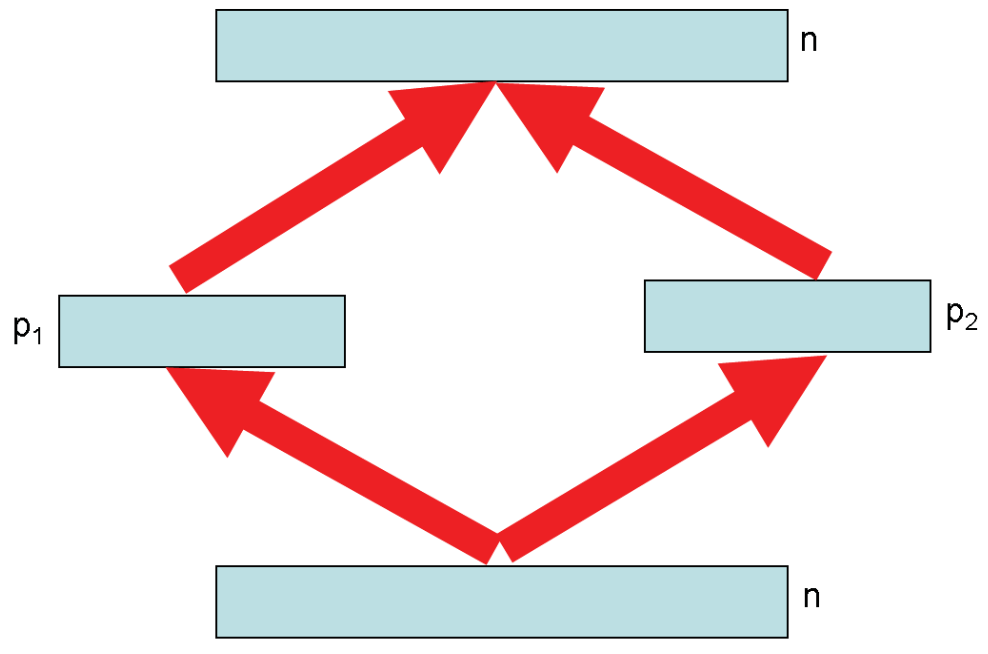
\includegraphics[width=0.4\textwidth]{./Images/Overcomplete_autoencoders.png}
        \caption{Horizontally combining autoencoder}
    \end{figure}
\end{center}

In this context of large hidden layers, in addition to vertical composition, there is also
a natural horizontal composition for autoencoders that can be used to create large hidden
layer representations simply by horizontally combining autoencoders. Two (or
more) autoencoders with architectures $n/p_1/n$ and $n/p_2/n$] can be trained and the hidden
layers can be combined to yield an expanded hidden representation of size $p_1 + p_2$ that
can then be fed to the subsequent layers of the overall architecture. Differences in the
p1 and p2 hidden representations could be introduced by many different mechanisms, for
instance using different learning algorithms, different initializations, different training samples, different learning rates, or different distortion measures.